%!TEX encoding = UTF-8 Unicode

\section*{Study area}

D\textsc{cca} is an intensively managed wetland located near Puxico, Missouri, managed by the Missouri Department of Conservation (\textsc{mdc}; Figure~\ref{fig:area_map}). The area totals 2,557 ha including a 728 ha shallow lake (Pool~1), 486 ha of actively managed bottomland hardwood forest (Pool~2 and Pool~3), and marsh units. The pool and forest areas provide habitat for Hooded Mergansers and Wood Ducks year around but particularly during their breeding season. The shallow lake known as Pool 1 serves as a large food source housing robust populations of fish and aquatic invertebrates. The bottomland hardwood forest provides nesting habitat and is seasonally flooded in the winter to provide roosting and foraging habitat. The area is bordered by the federally managed Mingo National Wildlife Refuge with another 8,500 ha of similar habitat.  Two other nearby \textsc{mdc} conservation areas, Ten Mile Pond and Otter Slough are managed in conjunction with \textsc{dcca} to provide wintering and spring nesting waterfowl habitat across southeastern Missouri. 

\afterpage{%
\begin{figure}[p!]
	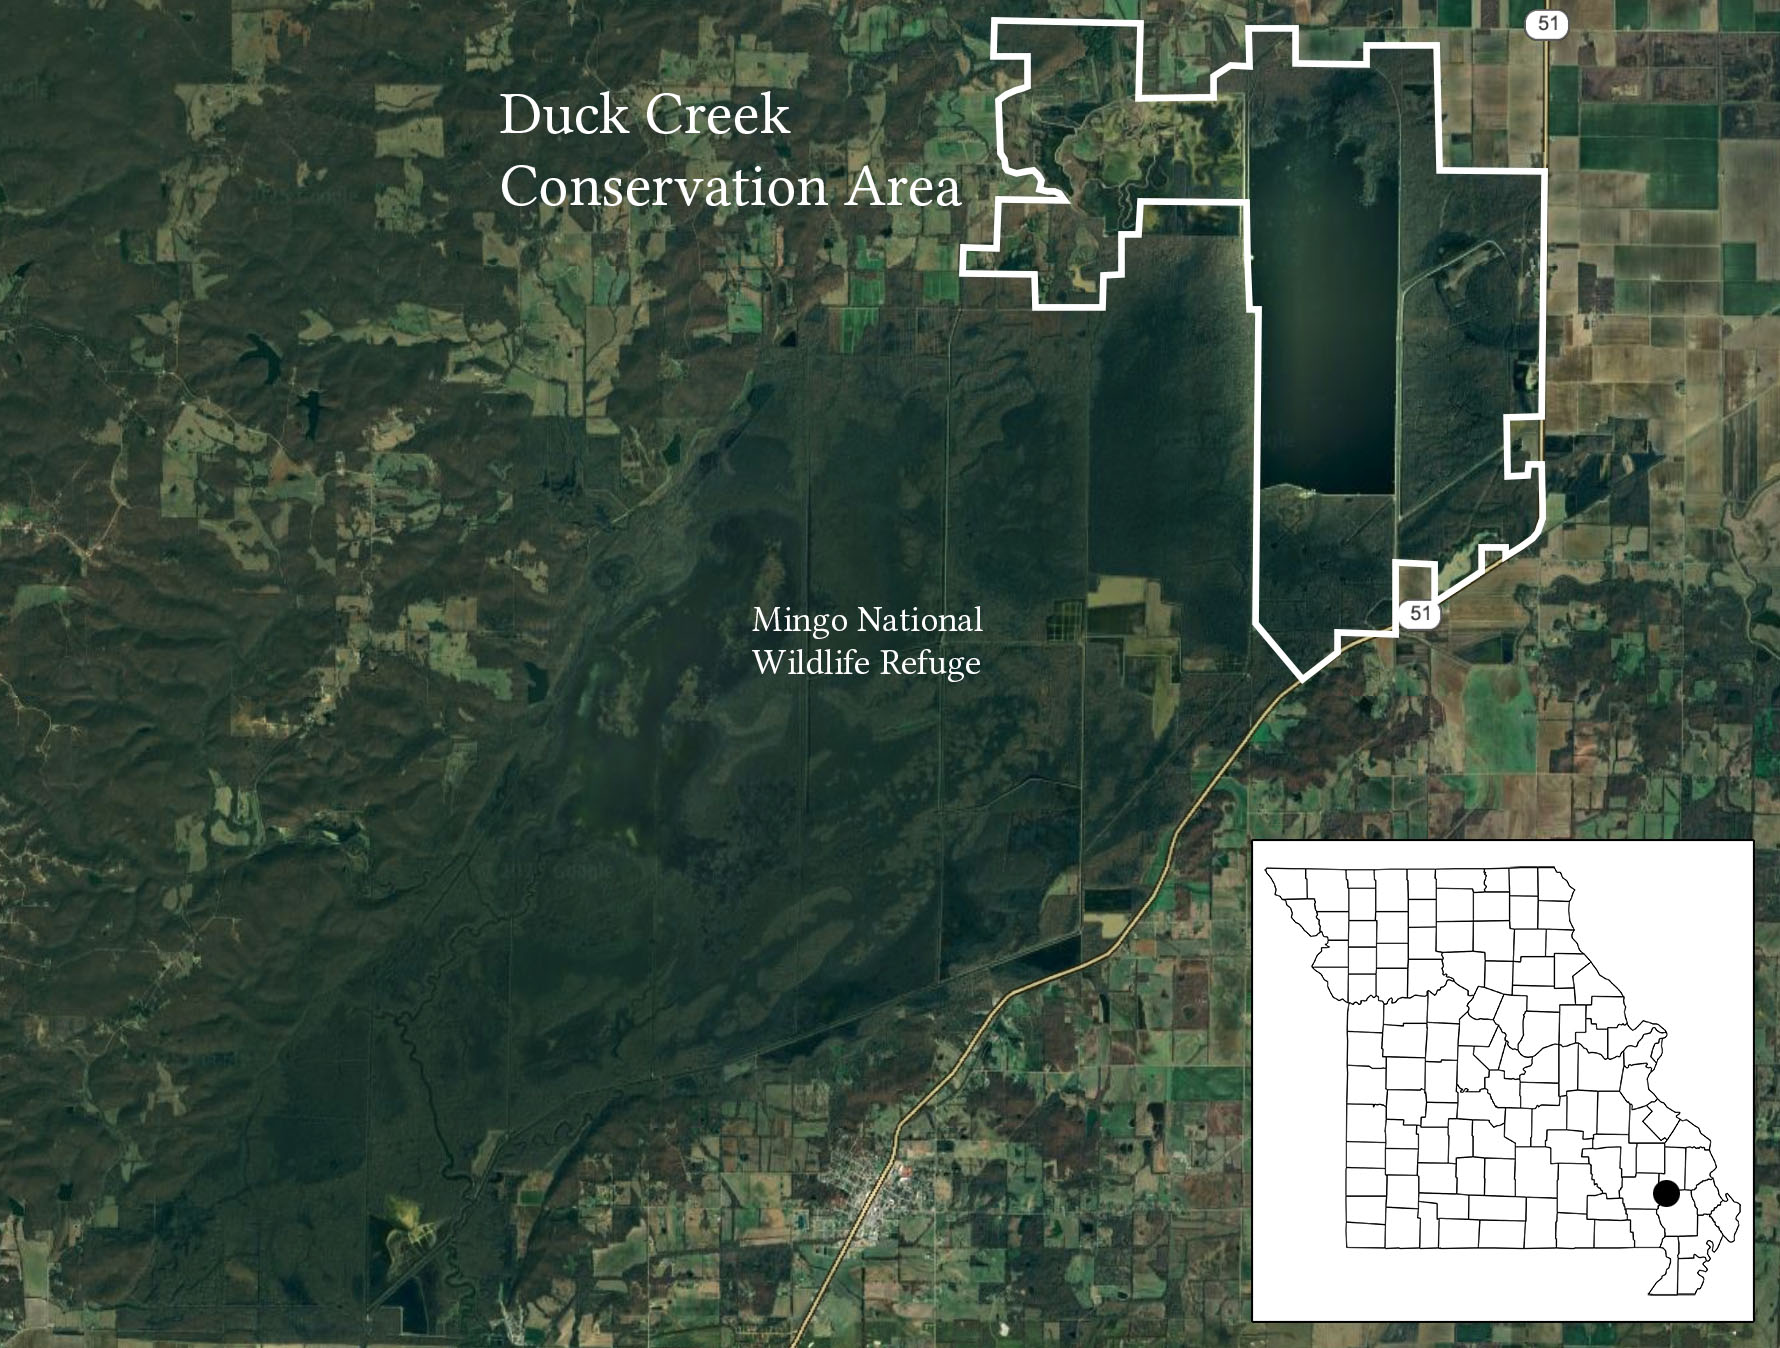
\includegraphics[width=\textwidth]{area_map}
	\caption[Duck Creek Conservation Area in southeast Missouri]{Duck Creek Conservation area and Mingo National Wildlife Refuge in Southeast Missouri. The approximate boundary of Duck Creek Conservation Area is outlined in white.}
	\label{fig:area_map}
\end{figure}
\clearpage}
 


\section*{Data collection}

The \textsc{mdc} maintains about 100 nest boxes for Hooded Merganser and Wood Duck reproduction, distributed around Pools 1–3.  Ten nest boxes were selected randomly from each pool for a total of 30 boxes to monitor hatching success (Figure~\ref{fig:nest_box_map}).  Pool~1  boxes were typically located along wider, deeper ditches with little tree cover. Pool~2 boxes were located along much narrower, shallower ditches with moderate tree cover. Pool~3 boxes were located on a mixture of broad flooded woods, narrow to wide ditches with heavy tree cover. For each box, tree cover and number of nearby boxes was measured using onXmaps GPS software (OnX Hunt 2025). Boxes were checked weekly from 23 March through 28 June 2024 to measure water width and depth, count eggs laid, hatched, abandoned, or lost, and identify both egg and nesting hen species. Weekly monitoring of nests ensured eggs were counted after hatching and to reduce the chance of eggshells being destroyed before counting. 

\afterpage{%
\begin{figure}[p!]
	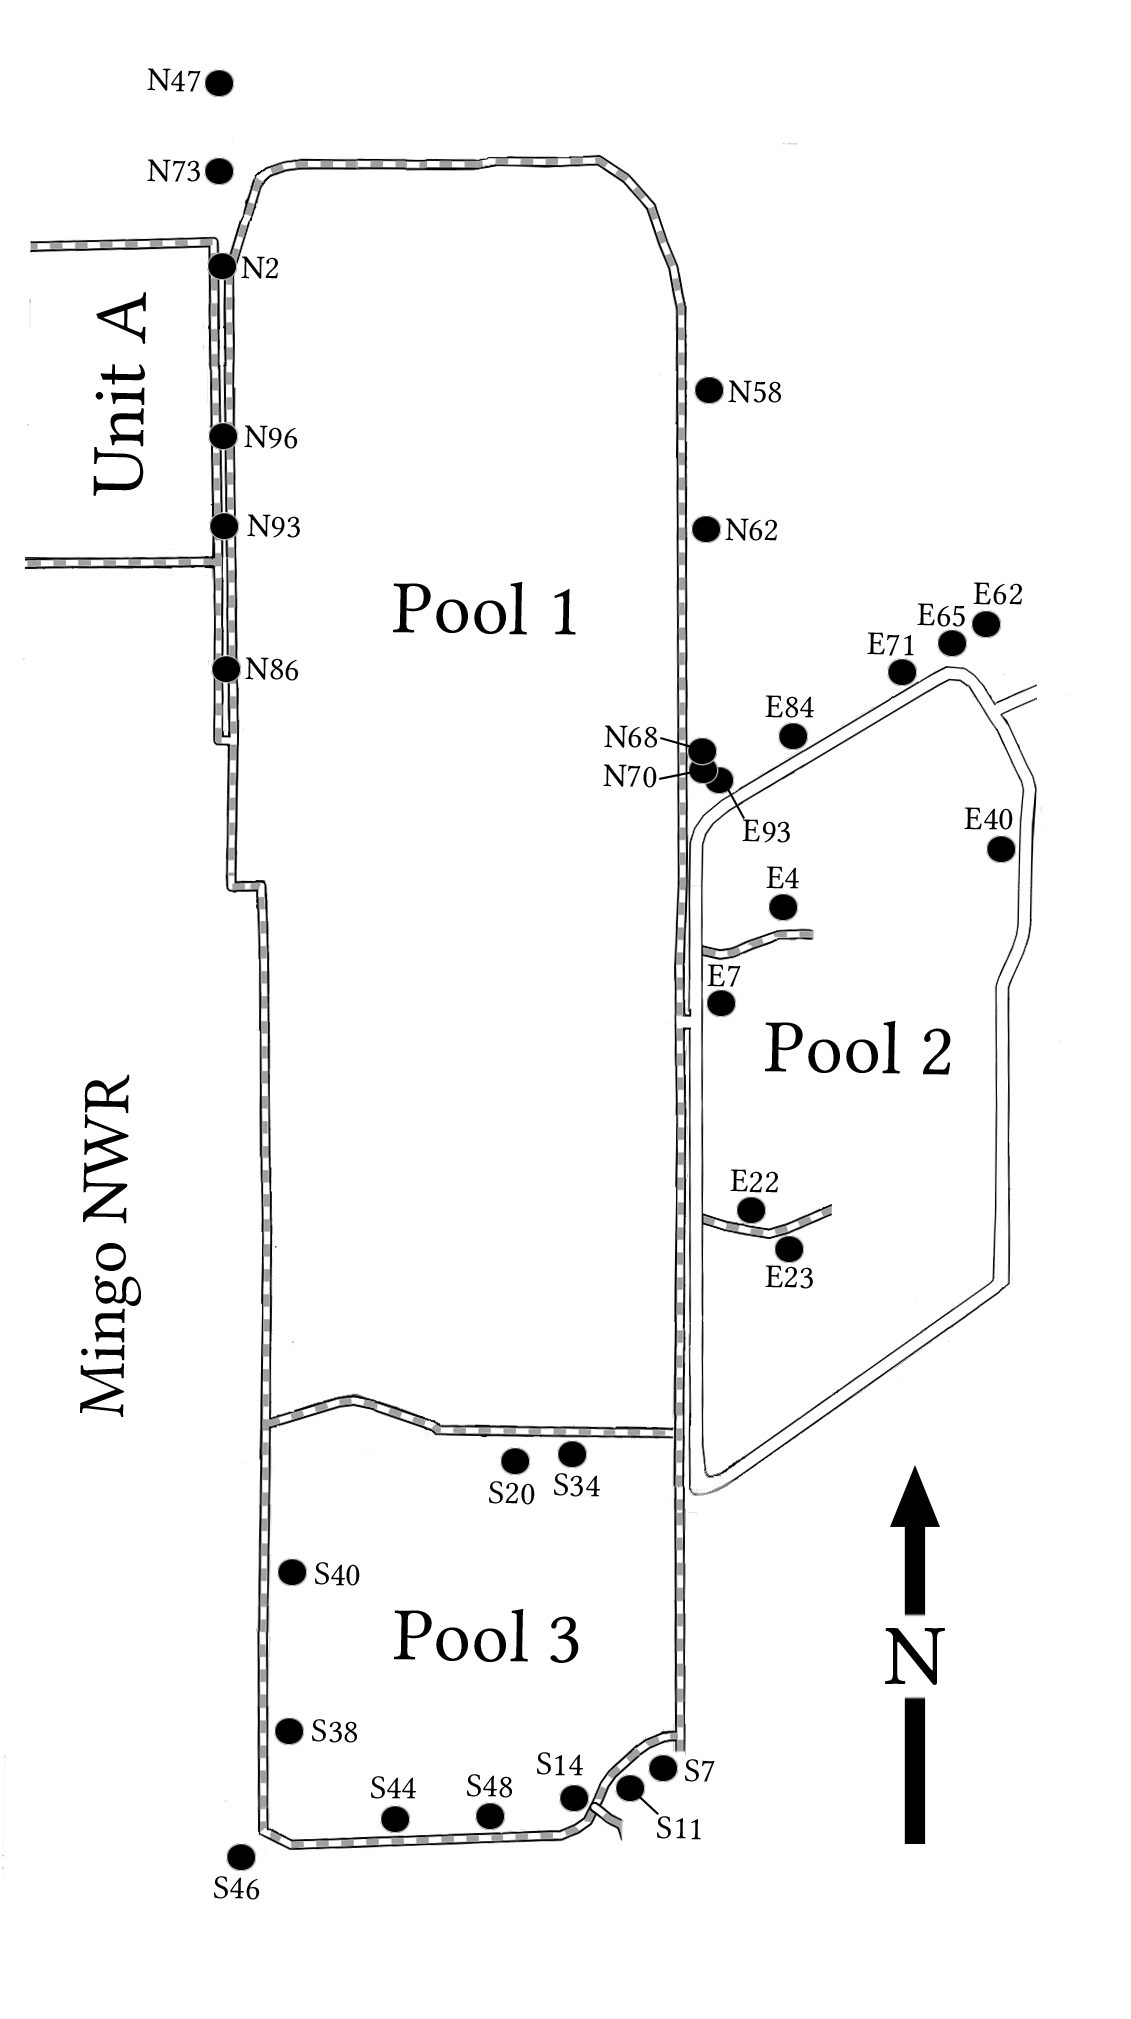
\includegraphics[height=0.85\textheight]{nest_box_map}
	\caption[Map showing location of 30 duck nest boxes sampled for this study]{Map showing location of 30 duck nest boxes sampled for this study. Boxes in the north section are located adjacent to Pool 1. Boxes in the east section are located adjacent to Pool 2. Boxes in the south section are located adjacent to Pool 3.}
	\label{fig:nest_box_map}
\end{figure}
\clearpage}
 

Dump nesting within and between species was determined by inspecting the size, shape, and color of eggs present. Wood Duck eggs are relatively small, tan to brown, and oblong. By comparison, Hooded Merganser eggs are larger, paler, and rounder (Figure~\ref{fig:wood_duck_nest}). Dump nesting by conspecifics was determined by additional eggs being counted at later inspections or by eggs lagging in development stage upon first inspection. Development stage was determined by egg candling, a process where a dark tube is used to observe light passing through an egg (Figure~~\ref{fig:candling_example}) to observe the embryo. The shape and position of the developing embryo can be used to estimate the age of the egg in days (Jalaludeen et al. 2022, Figure~\ref{fig:egg_candling}).  If an egg was developmentally behind others in the nest it was considered dumped. In nests with only Wood Duck eggs or where heterospecific dump nesting was present, two eggs were candled to establish the age of the nest. In nests with only Hooded Merganser eggs, eggs were candled until dump nesting was found or all eggs were candled. Wood Duck nests were not able to be fully candled and Hooded Merganser nests were stopped once dumping was found due to permit restrictions.  

\afterpage{%
\begin{figure}[p!]
	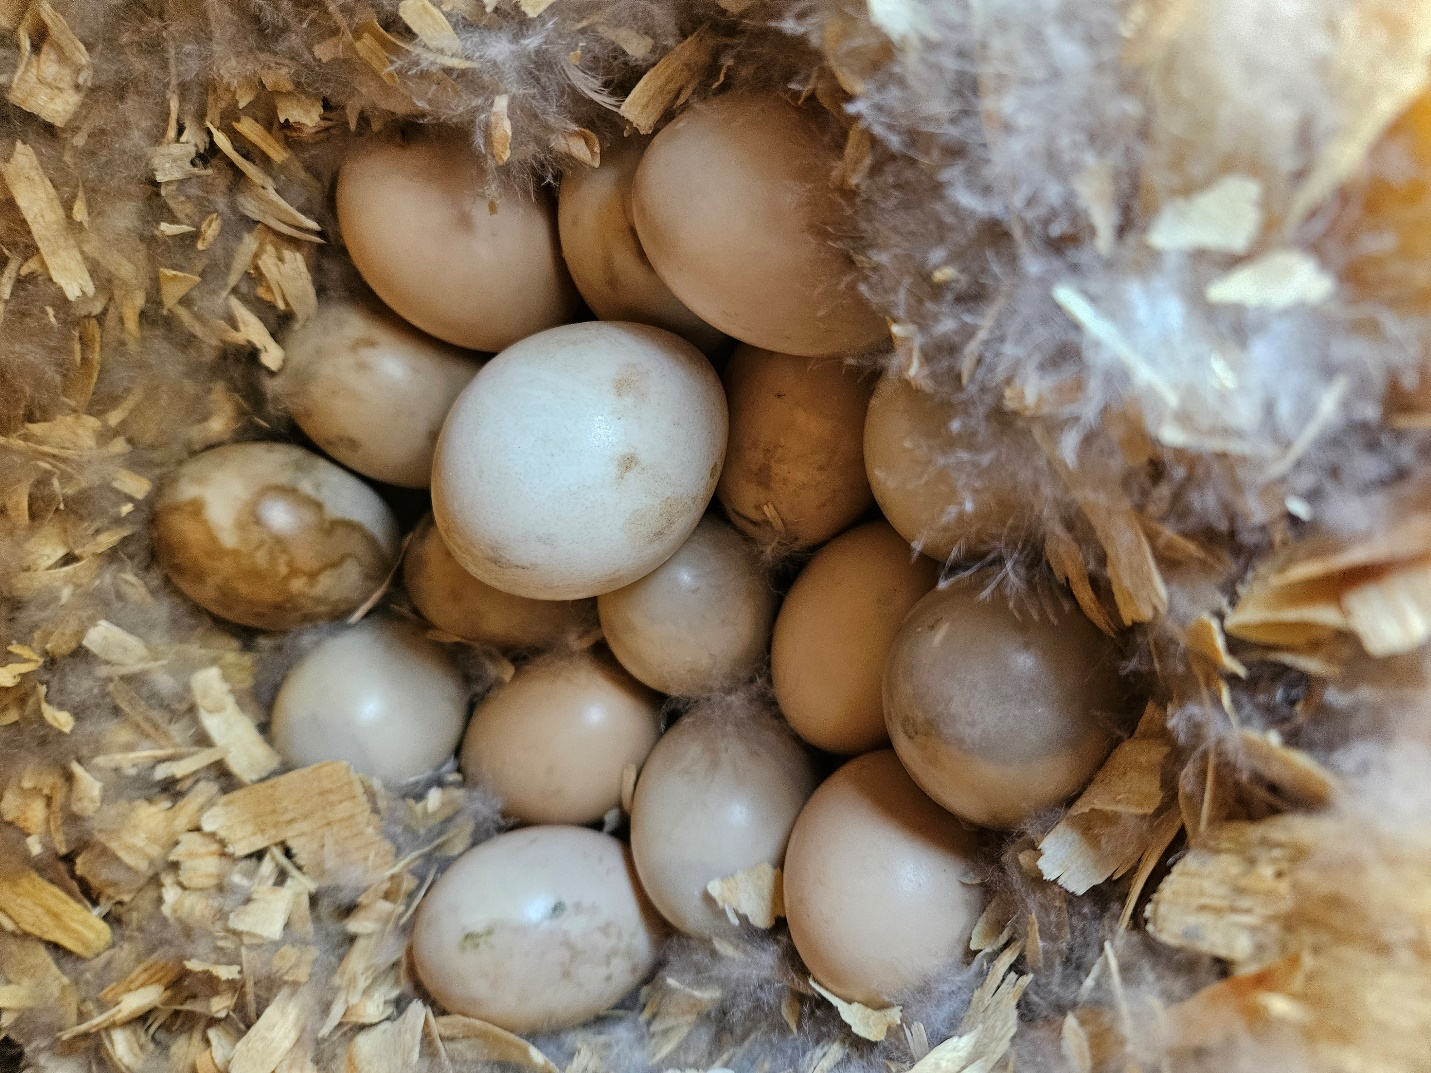
\includegraphics[width=\textwidth]{wood_duck_nest}
	\caption[Photograph of a Wood Duck nest with a dumped Hooded Merganser egg on top]{Photograph of a Wood Duck nest with a dumped Hooded Merganser egg on top in box E65 at Duck Creek Conservation Area, Puxico, Missouri. Wood duck eggs are visually smaller, browner, and more oblong where the Hooded Merganser egg is slightly larger, paler, and rounder by comparison. Photo by Frank J.\,Irovic. }
	\label{fig:wood_duck_nest}
\end{figure}
\clearpage}
 

\afterpage{%
\begin{figure}[p!]
	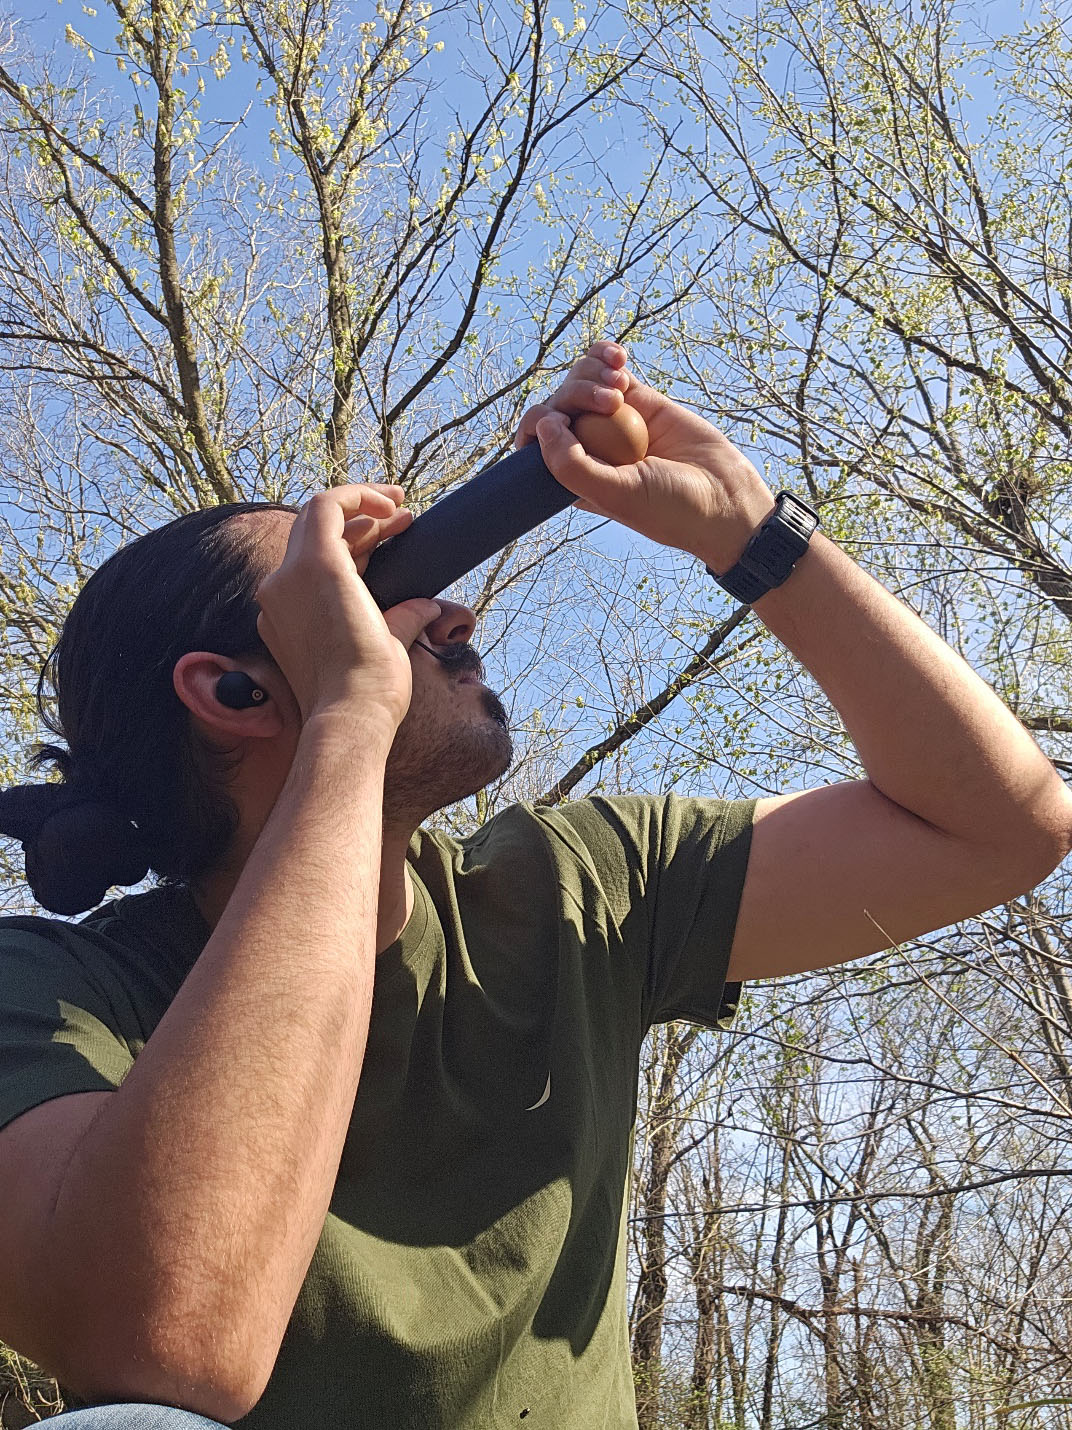
\includegraphics[width=0.99\textwidth]{candling_example}
	\caption[Photograph demonstrating a representation of egg candling]{Photograph demonstrating a representation of egg candling using a chicken egg. Photo by Frank J.~Irovic.}
	\label{fig:candling_example}
\end{figure}
\clearpage}
 

\afterpage{%
\begin{figure}[p!]
	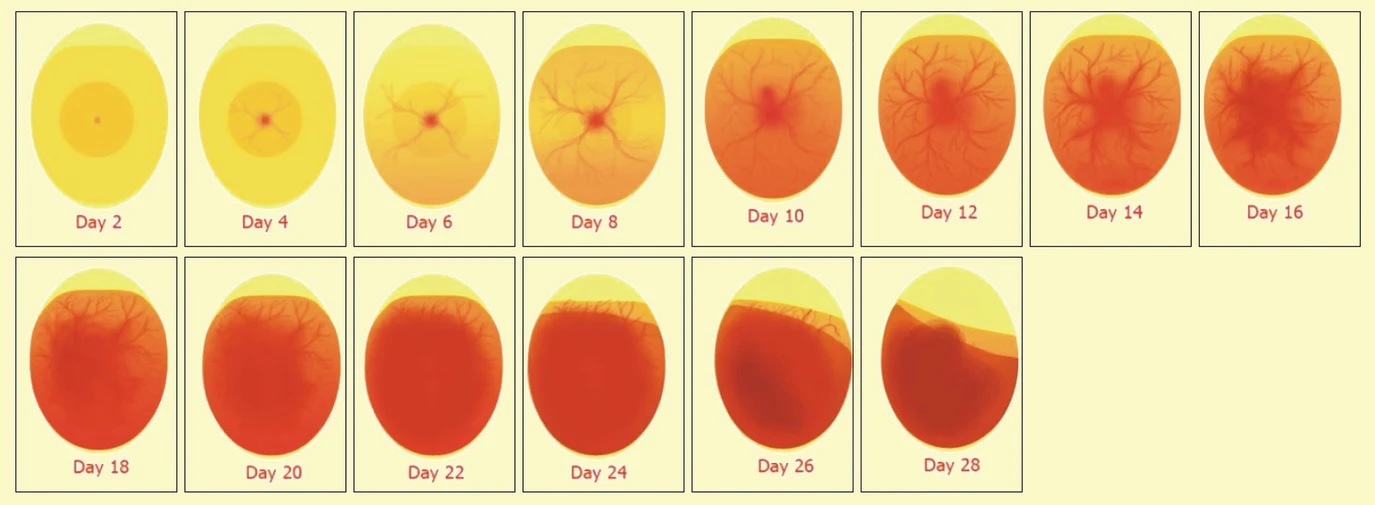
\includegraphics[width=\textwidth]{egg_candling}
	\caption[Developmental diagram of embryo development in ducks]{Developmental diagram of embryo development in ducks. Days indicate days since the start of incubation. Hatching occurs at approximately 28 to 29 days. Figure modified from Jalaludeen et~al.\,2022.}
	\label{fig:egg_candling}
\end{figure}
\clearpage}
 

At each weekly inspection, width and depth of water nearest the nest box was measured manually and the box was photographed. At the initial inspection of a nest its eggs would be identified, counted, and candled. Additionally, at the initial and all subsequent inspections eggs were counted to identify dumping or predation loss and the nests were photographed. This ensured that any changes to the nest could be confirmed in weekly intervals. Eggs were considered hatched, lost, or abandoned. Eggs that were present during the inspection prior to hatching were confirmed through counting eggshells after the nest was hatched. Any eggs that were found to have gone missing between weekly inspections were counted as lost to predation.  Any eggs that remained intact after the nest hatched were considered abandoned.  

\section*{Data analysis}

R statistical computing software version 4.4.1 (R Core Team 2024) was used for analysis. A\textsc{nova} or \textit{t}-tests from base R were used to test for significant differences of habitat variables among sections or egg-related variables (e.g. hatching) between species. If significant differences of habitat variables were identified among sections, then Tukey's Honestly Signficant Difference (\textsc{hsd}) test was used  for post-hoc determination of which sections were significantly different from the others. 

%A master dataset was compiled with all variables recorded for each of the thirty boxes. This was then edited down into an analysis dataset featuring box number, box section, species, number of eggs hatched, log of tree coverage, and the modal width and depth of the nearest water while the nest was active. Log of tree coverage was used as the values for coverage were significantly larger than the other variables resulting in points being clustered close together without visual separation. Log coverage in contrast maintained the relative distribution of points to each other while spreading them further apart. This allowed for a visually clearer figure and easier data interpretation. 

Non-metric multidimensional scaling \textsc{(nmds)} analysis was performed in R using the meta\textsc{mds} function from vegan 2.6-8 (Oksanen et al. 2025). N\textsc{mds} is an ordination technique that represents multiple variables on two to three axes while preserving the ordering of objects (e.g., nest boxes) along those variables (Rabinowitz 1975, Legendre and Legendre 1998). Bray-Curtis distance was used to estimate the ordering relationship among nest boxes based on number of eggs hatched, water width and depth, and tree coverage. Only data from nest boxes with attempted nesting events were used in the \textsc{nmds} analysis. 


